\thispagestyle{toancuabinone}
\pagestyle{toancuabi}
\everymath{\color{toancuabi}}
%\blfootnote{$^1$\color{toancuabi}Đại học Thăng Long.}
\graphicspath{{../toancuabi/pic3/}}
\begingroup
\AddToShipoutPicture*{\put(0,616){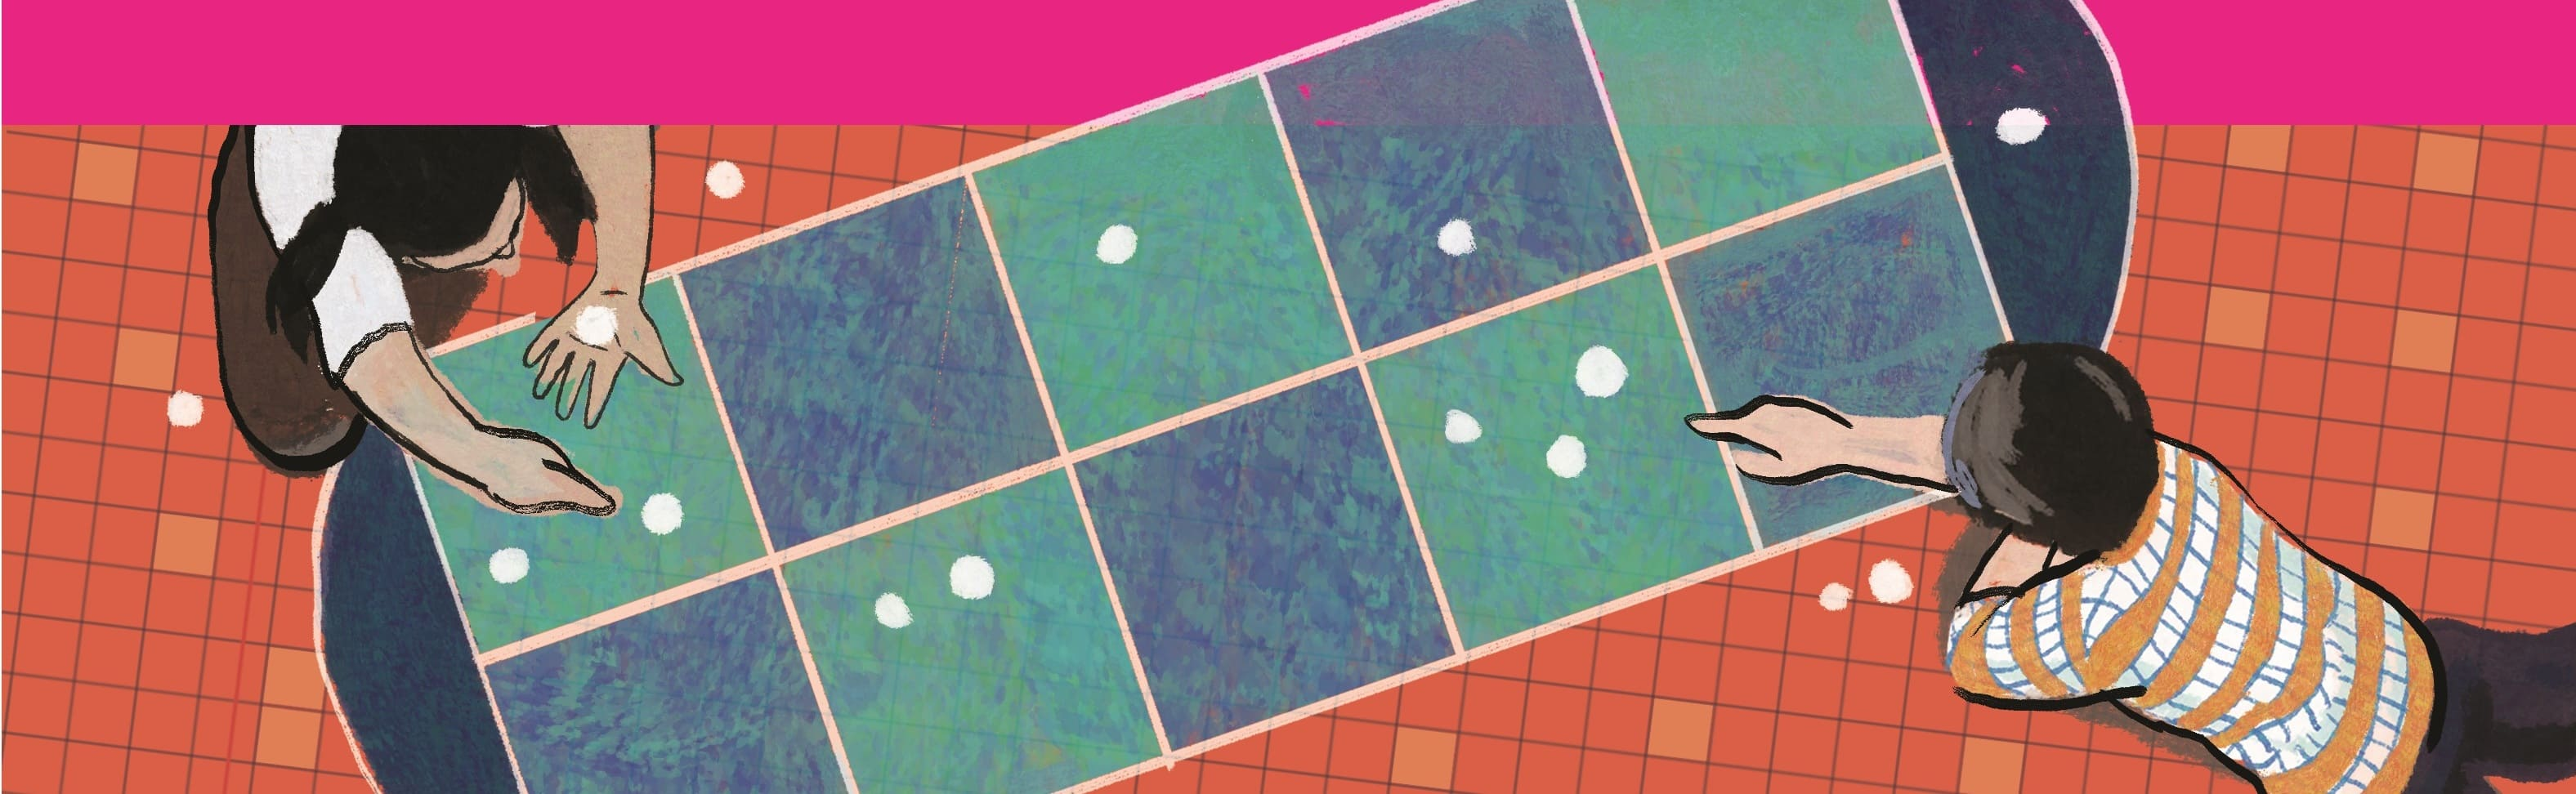
\includegraphics[width=19.3cm]{../bannertoancuabi}}}  
\AddToShipoutPicture*{\put(90,550){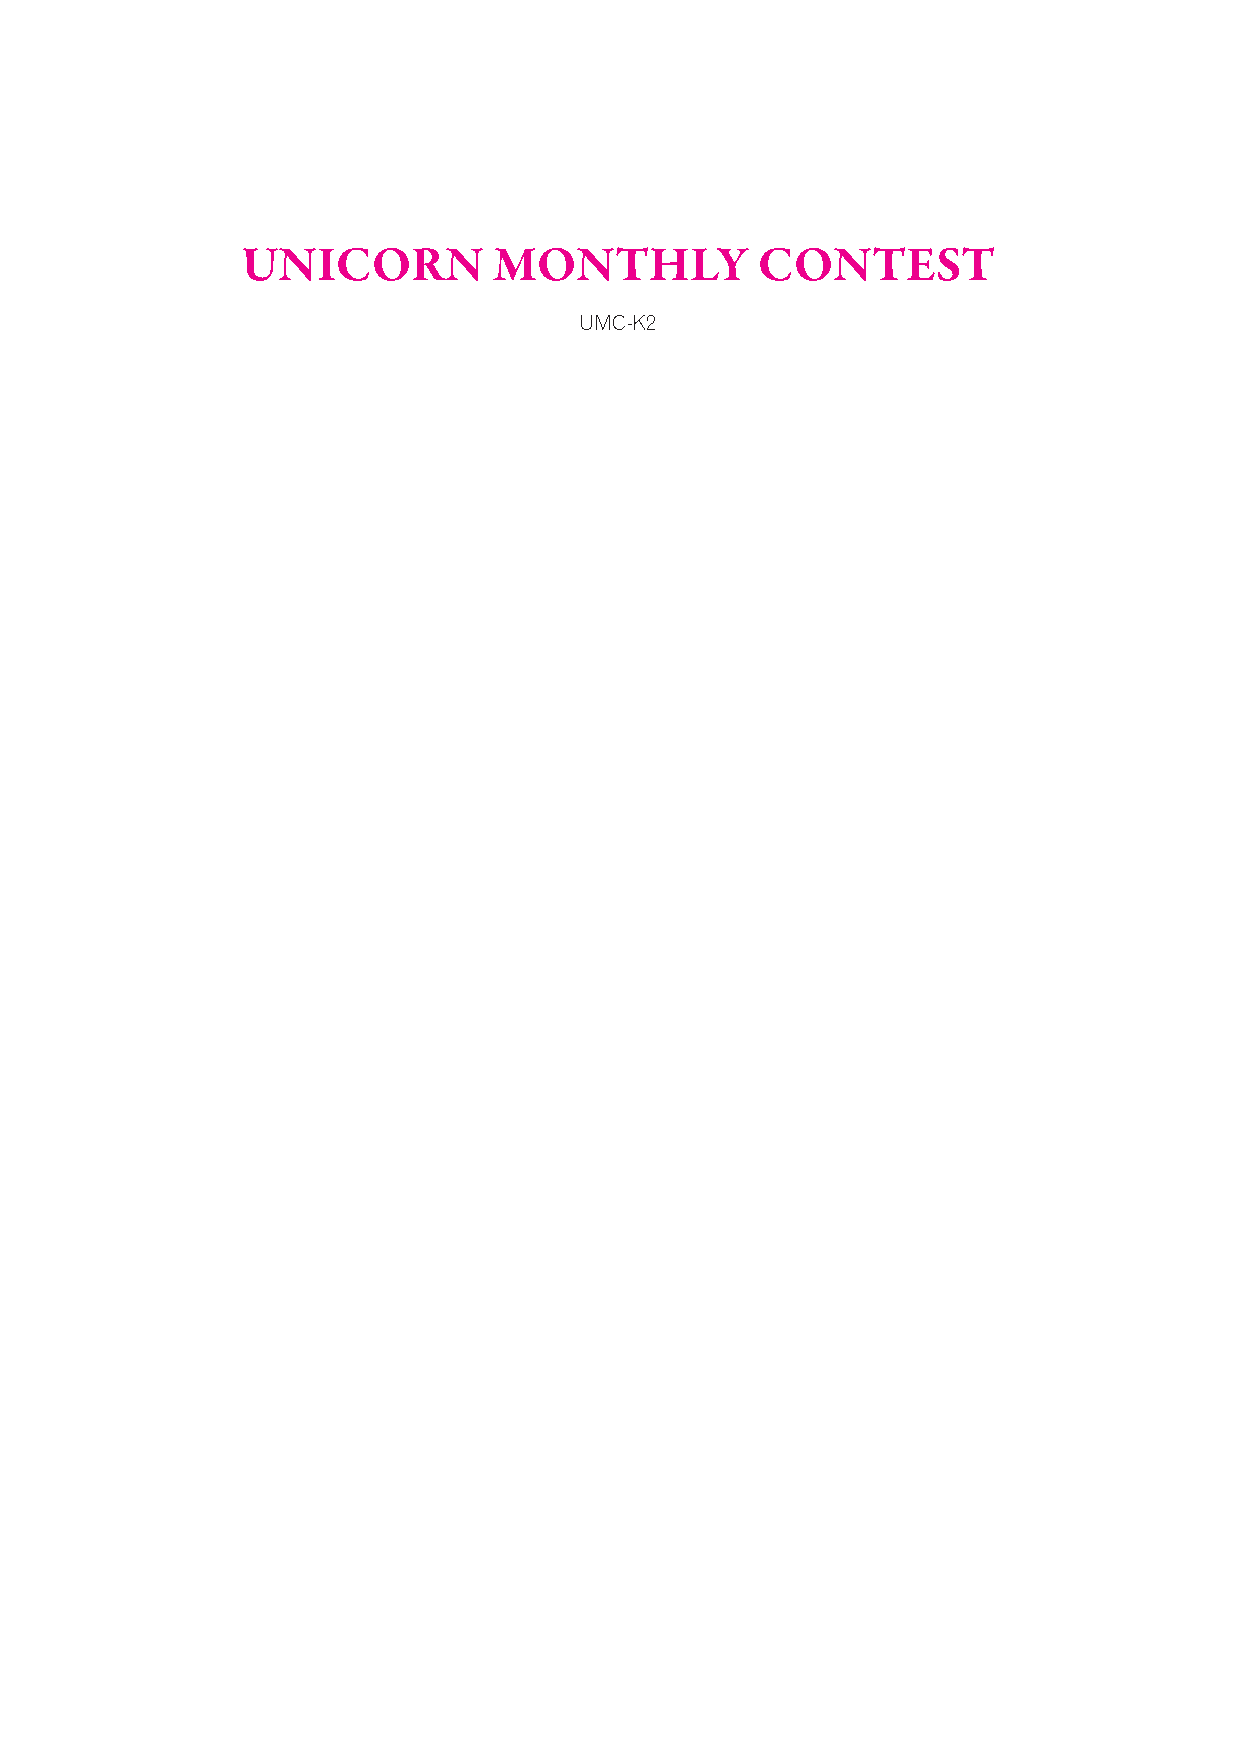
\includegraphics[scale=1]{../tieude1b.pdf}}} 
\centering
\endgroup
\vspace*{160pt}

\begin{multicols}{2}
	\textbf{\color{toancuabi}Bài} $\pmb{1.}$ Cho đa giác lồi $n$ cạnh có $65$ đường chéo. Tìm giá trị của $n$.
	\vskip 0.1cm
	\textbf{\color{toancuabi}Bài} $\pmb{2.}$ Tìm số nguyên dương $n$ sao cho $7n$ chia hết cho $n+1$.
	\vskip 0.1cm
	\textbf{\color{toancuabi}Bài} $\pmb{3.}$ Một tờ giấy hình tròn được vẽ các đường tròn màu xanh, đỏ và vàng cùng tâm. Nếu cắt dọc theo các đường màu xanh, bạn nhận được $10$ mảnh, nếu cắt dọc theo các đường màu đỏ bạn nhận được $12$ mảnh và nếu cắt theo các đường màu vàng bạn nhận được $18$ mảnh. Hỏi nếu cắt theo tất cả các đường cả xanh, đỏ, vàng thì bạn nhận được bao nhiêu mảnh giấy?
	\vskip 0.1cm
	\begin{figure}[H]
		\vspace*{-5pt}
		\centering
		\captionsetup{labelformat= empty, justification=centering}
		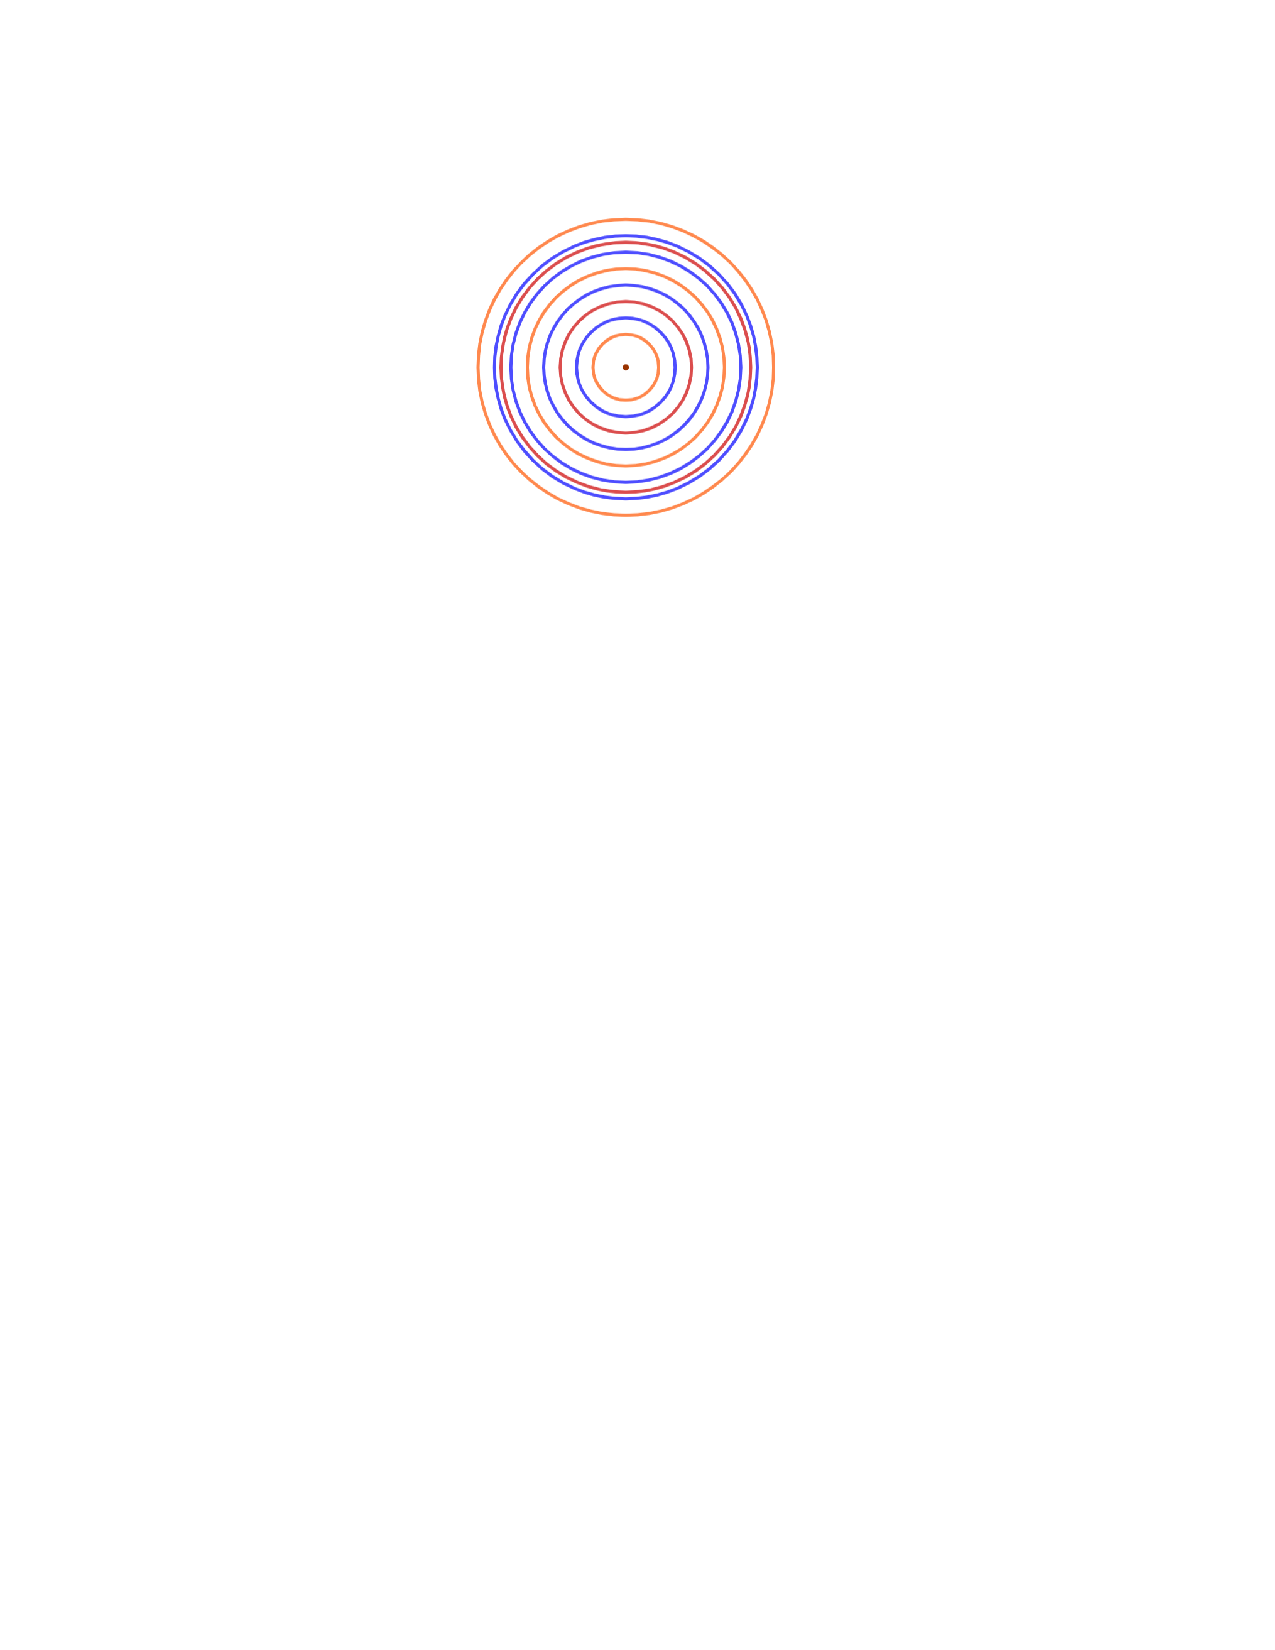
\includegraphics[width= 0.6\linewidth]{bai3}
		\caption{\small\textit{\color{toancuabi}Hình vẽ mang tính chất minh họa.}}
		\vspace*{-10pt}
	\end{figure}
	\textbf{\color{toancuabi}Bài} $\pmb{4.}$ Tìm số có $2$ chữ số $AB$ thỏa mãn điều kiện như
	phép tính bên.
	\begin{table}[H]
		\vspace*{-5pt}
		\centering
		\captionsetup{labelformat= empty, justification=centering}
		\begin{tabular}{ccc}
			&$A$&$B$\\
			$\times$& &$A$\\
			\hline
			$B$&$A$&$A$\\
		\end{tabular}	
		%		\caption{\small\textit{\color{}.}}
		\vspace*{-10pt}
	\end{table}
	\textbf{\color{toancuabi}Bài} $\pmb{5.}$ Trong vườn của bác nông dân có $2024$ cây đào. Có đúng một nửa số cây đào đang ra hoa và $\frac{1}{4}$ số cây đào đang ra quả (trong số đó có một số cây đang ra cả hoa và quả). Biết rằng có $1000$ cây đào chưa ra cả hoa lẫn quả. Hỏi có bao nhiêu cây đào đã ra cả hoa và quả?
	\vskip 0.1cm
	\textbf{\color{toancuabi}Bài} $\pmb{6.}$ Tình chữ số tận cùng của $A = 2^{2021} + 3^{2022} + 4^{2023} + 7^{2024.}$
	\vskip 0.1cm
	\textbf{\color{toancuabi}Bài} $\pmb{7.}$ Câu lạc bộ tem có $40$ thành viên. Có $25$ người có không ít hơn $25$ cái tem và có $26$ người có ít hơn $26$ cái tem. Hỏi có bao nhiêu người có đúng $25$ cái tem?
	\vskip 0.1cm
	\textbf{\color{toancuabi}Bài} $\pmb{8.}$ Trên bảng ghi $21$ số chẵn liên tiếp. Bạn Phong xóa đi $1$ số và thấy tổng của các số còn lại bằng $2024$. Hỏi Phong đã đi xóa đi số nào?
	\vskip 0.1cm
	\textbf{\color{toancuabi}Bài} $\pmb{9.}$ Cho hình lập phương $ABCDEFGH$ như hình vẽ. Tính giá trị của góc $BDE$ theo độ
	\begin{figure}[H]
		\vspace*{-5pt}
		\centering
		\captionsetup{labelformat= empty, justification=centering}
		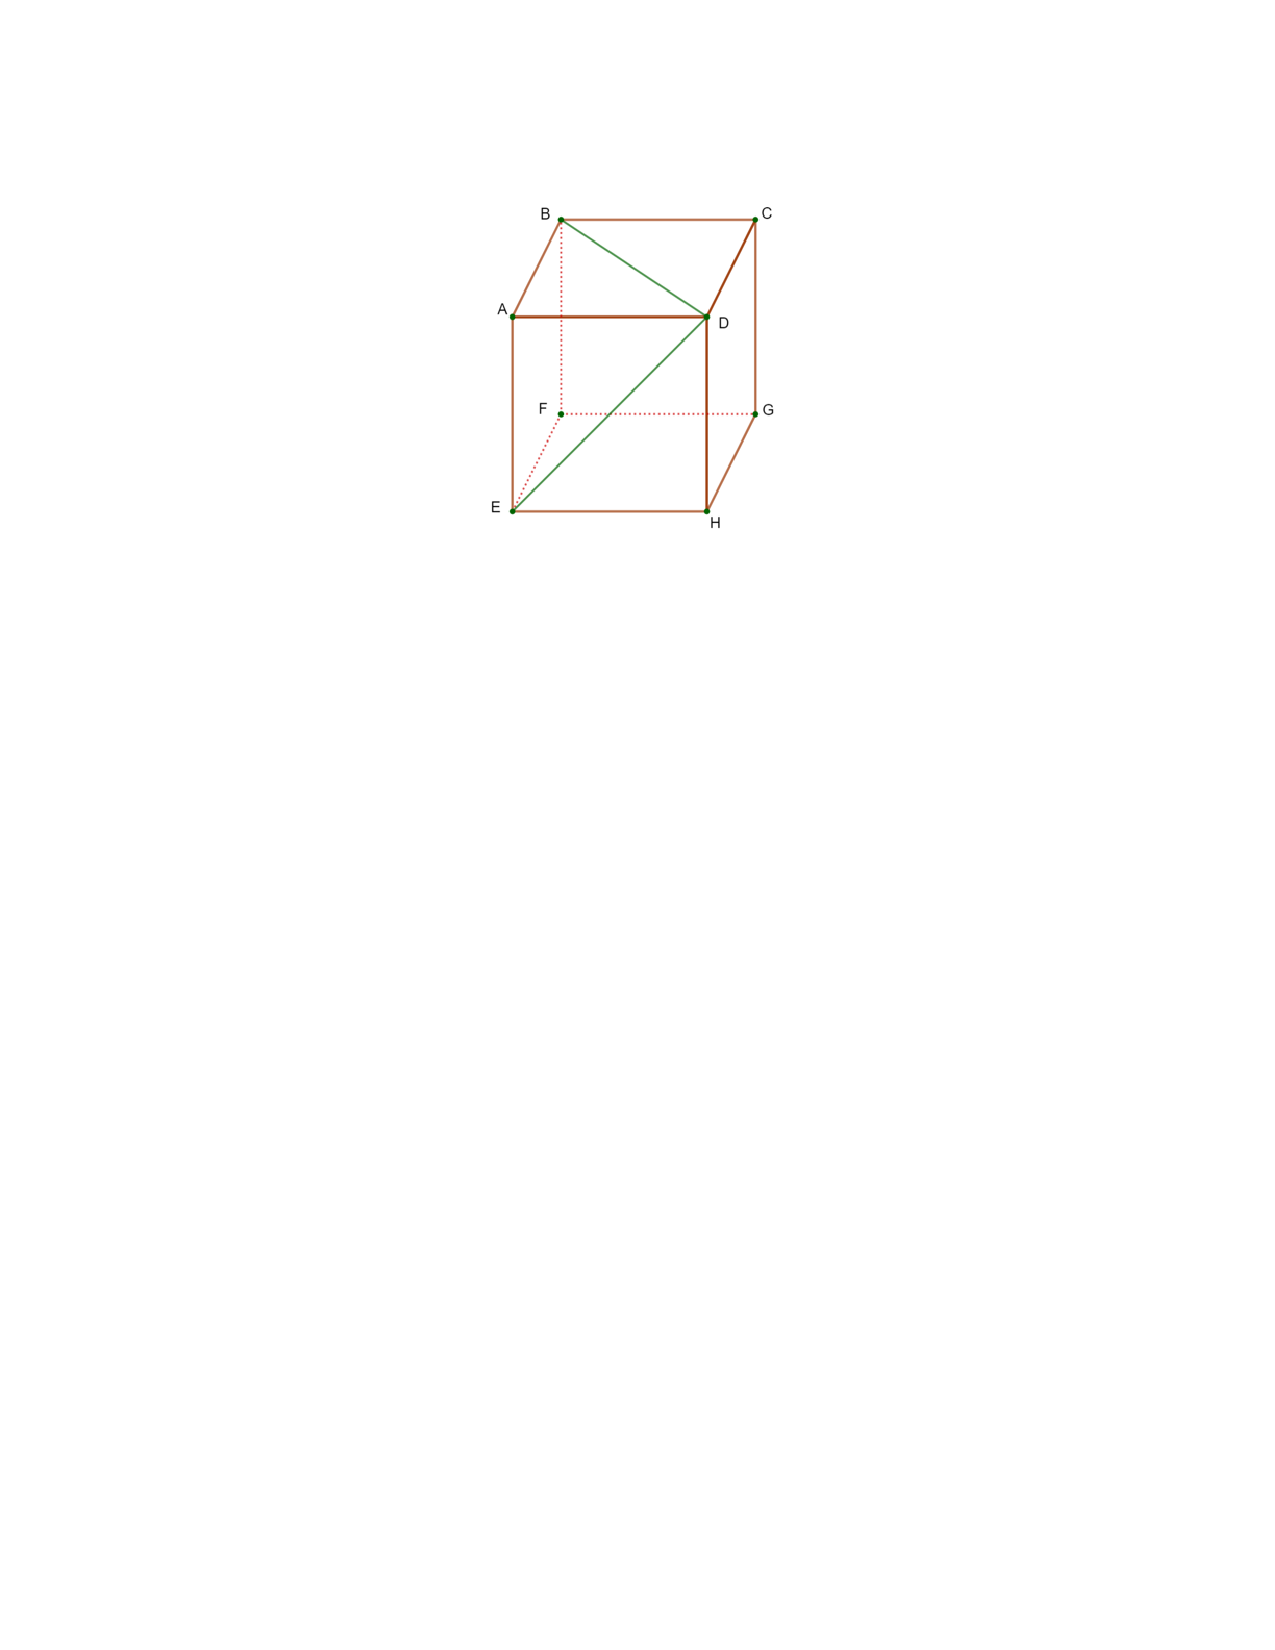
\includegraphics[width= 0.7\linewidth]{bai9k2}
		%		\caption{\small\textit{\color{}}}
		\vspace*{-10pt}
	\end{figure}
	\textbf{\color{toancuabi}Bài} $\pmb{10.}$ Hai tam giác đều $ABC$ và $MNP$ có
	các cạnh tương ứng song song với nhau, tam giác $ABC$ có $3$ cạnh tiếp xúc với đường tròn tâm $O$ và tam giác $MNP$ có $3$ đỉnh nằm trên đường tròn đó. Biết diện tích tam giác $ABC$ bằng $60$ cm$^2$. Tam giác $MNP$ có diện tích
	bằng bao nhiêu cm$^2$?
	\begin{figure}[H]
		\vspace*{-5pt}
		\centering
		\captionsetup{labelformat= empty, justification=centering}
		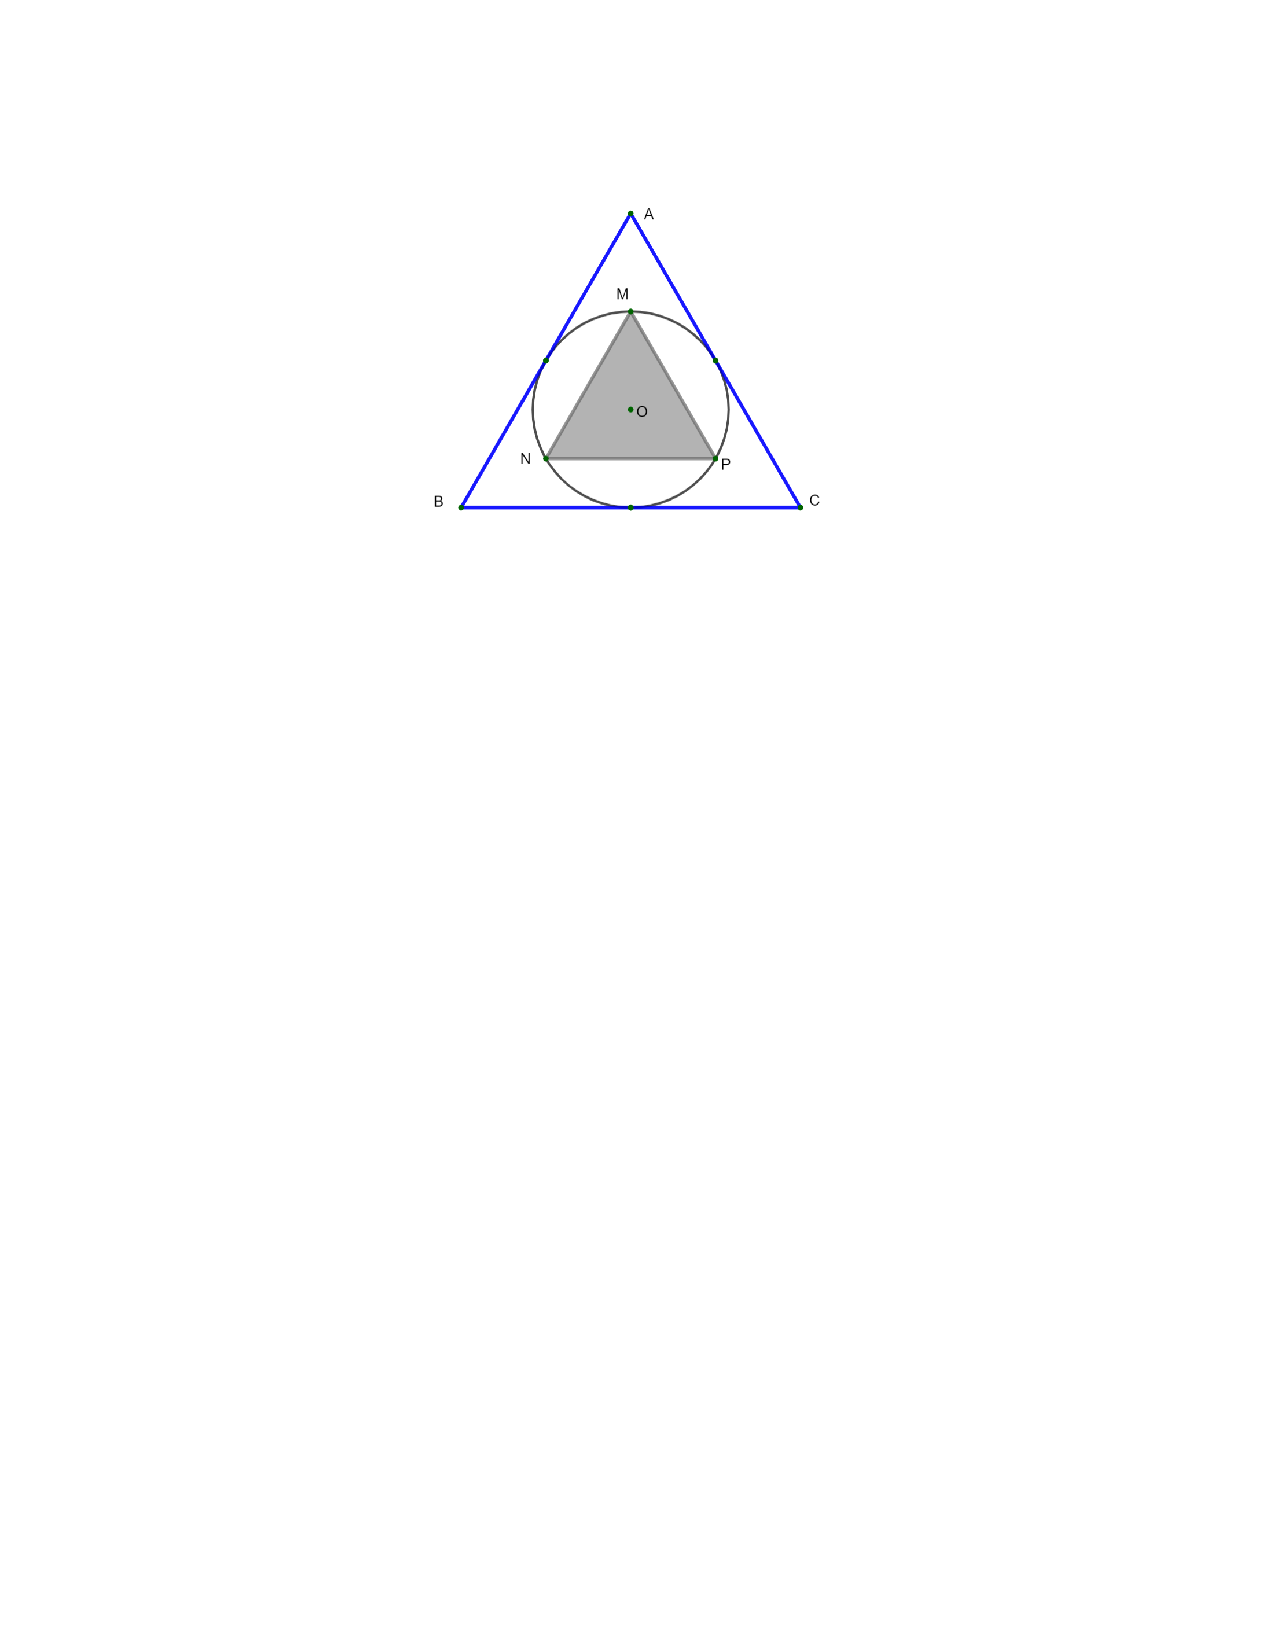
\includegraphics[width= 0.7\linewidth]{bai10k2}
		%		\caption{\small\textit{\color{}}}
		\vspace*{-10pt}
	\end{figure}
	\textbf{\color{toancuabi}Bài} $\pmb{11.}$ Có $15$ bạn nhỏ vào rừng hái nấm, các bạn hái được tổng cộng $106$ cái nấm và không có $2$ bạn nào hái được số nấm bằng nhau. Hỏi bạn hái nhiều nấm nhất hái được bao nhiêu cái nấm?
	\vskip 0.1cm
	\textbf{\color{toancuabi}Bài} $\pmb{12.}$ Một cái khóa số có mã gồm $3$ chữ số với các thông tin như hình bên. Bạn hãy phá khóa và cho biết mã của khóa là số nào?
	\begin{figure}[H]
		\vspace*{-5pt}
		\centering
		\captionsetup{labelformat= empty, justification=centering}
		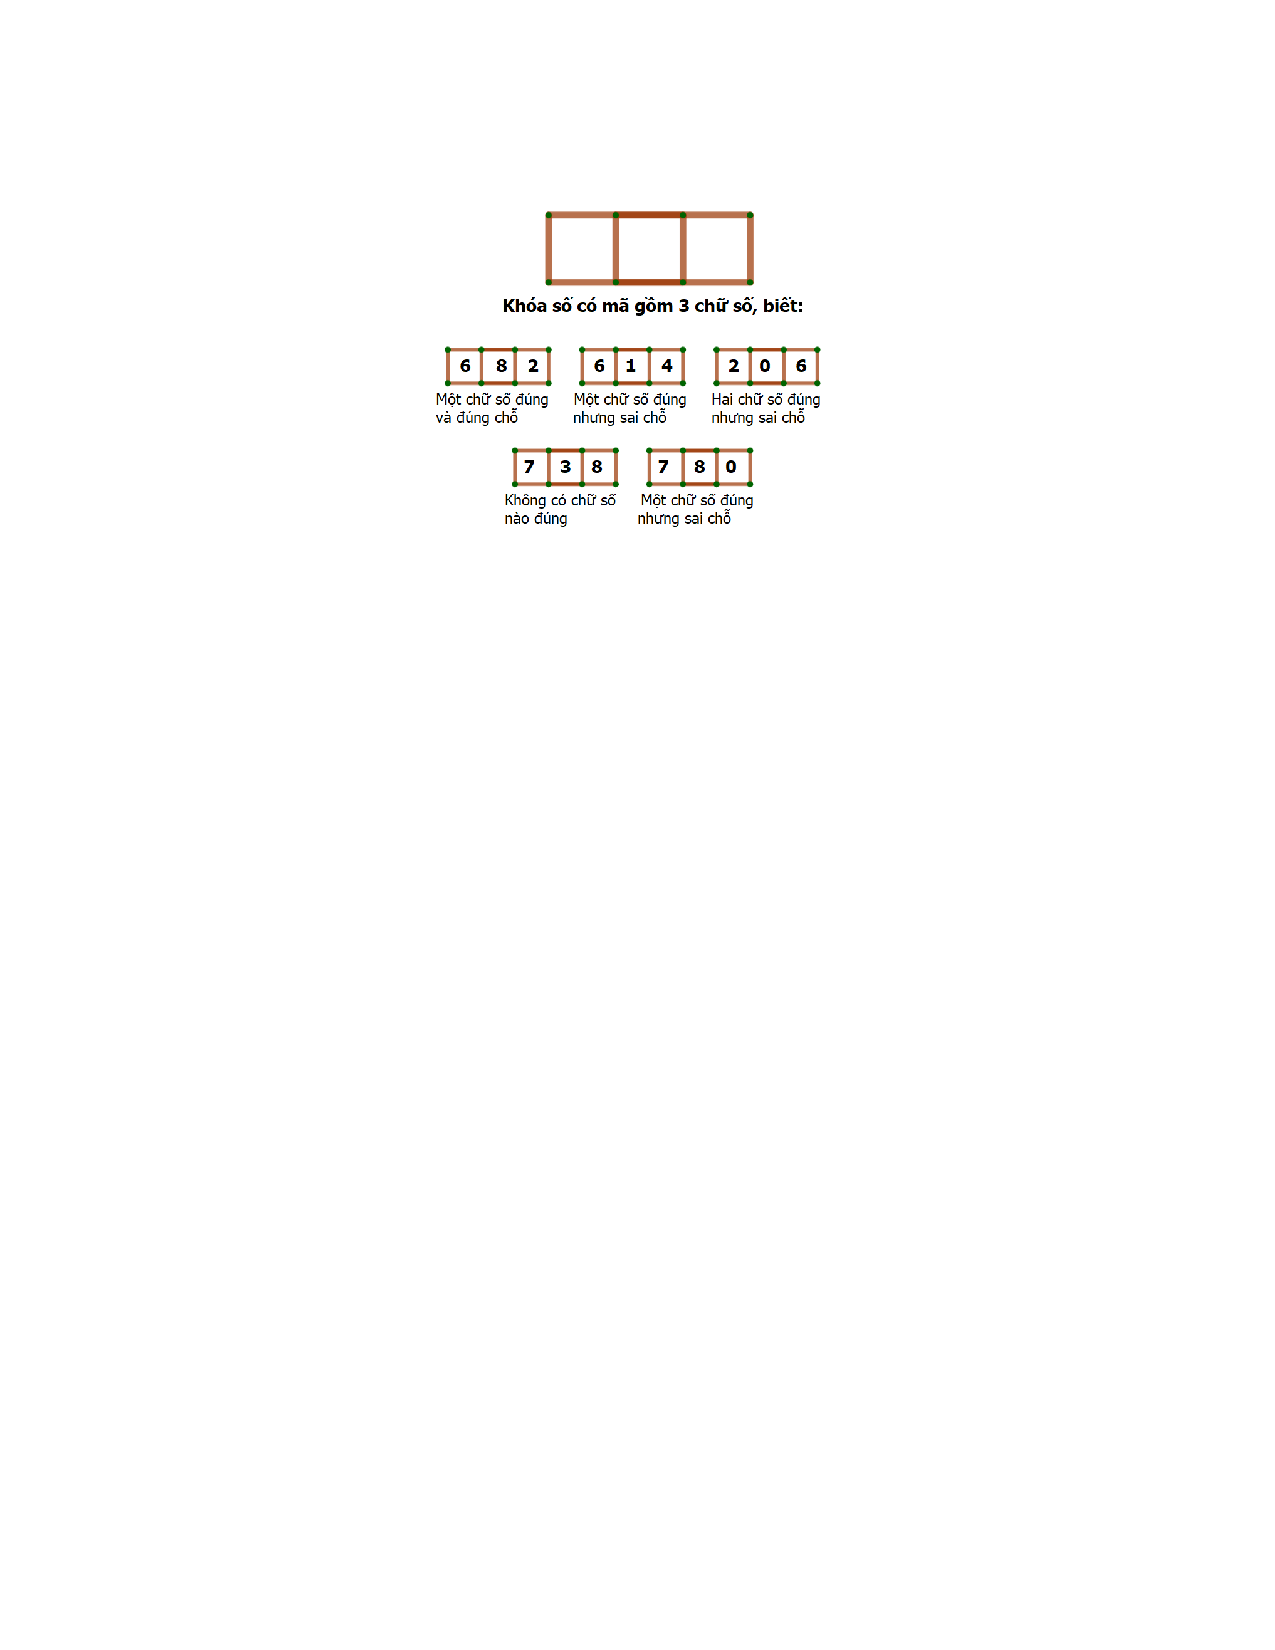
\includegraphics[width= 1\linewidth]{bai12}
		%		\caption{\small\textit{\color{}}}
		\vspace*{-15pt}
	\end{figure}
	\textbf{\color{toancuabi}Bài} $\pmb{13.}$ Tính giá trị của $S$.
	\begin{align*}
		S =& \frac{1}{1\times 2 \times 5} + \frac{1}{2\times 5 \times 6} + \frac{1}{6\times9\times 10} \\
		&+ \cdots + \frac{1}{26 \times 29 \times 30} + \frac{1}{29\times 30 \times 33}
	\end{align*}
	\textbf{\color{toancuabi}Bài} $\pmb{14.}$ Cho tam giác $ABC$ có diện tích bằng $60$ cm$^2$ như hình vẽ. Biết $BD=DE=EC$, $AF=FC$, $AD$ và $AE$ cắt $BF$ tại $H$ và $G$. Tính diện tích tam tứ giác $DEGH$
	\begin{figure}[H]
		\vspace*{-5pt}
		\centering
		\captionsetup{labelformat= empty, justification=centering}
		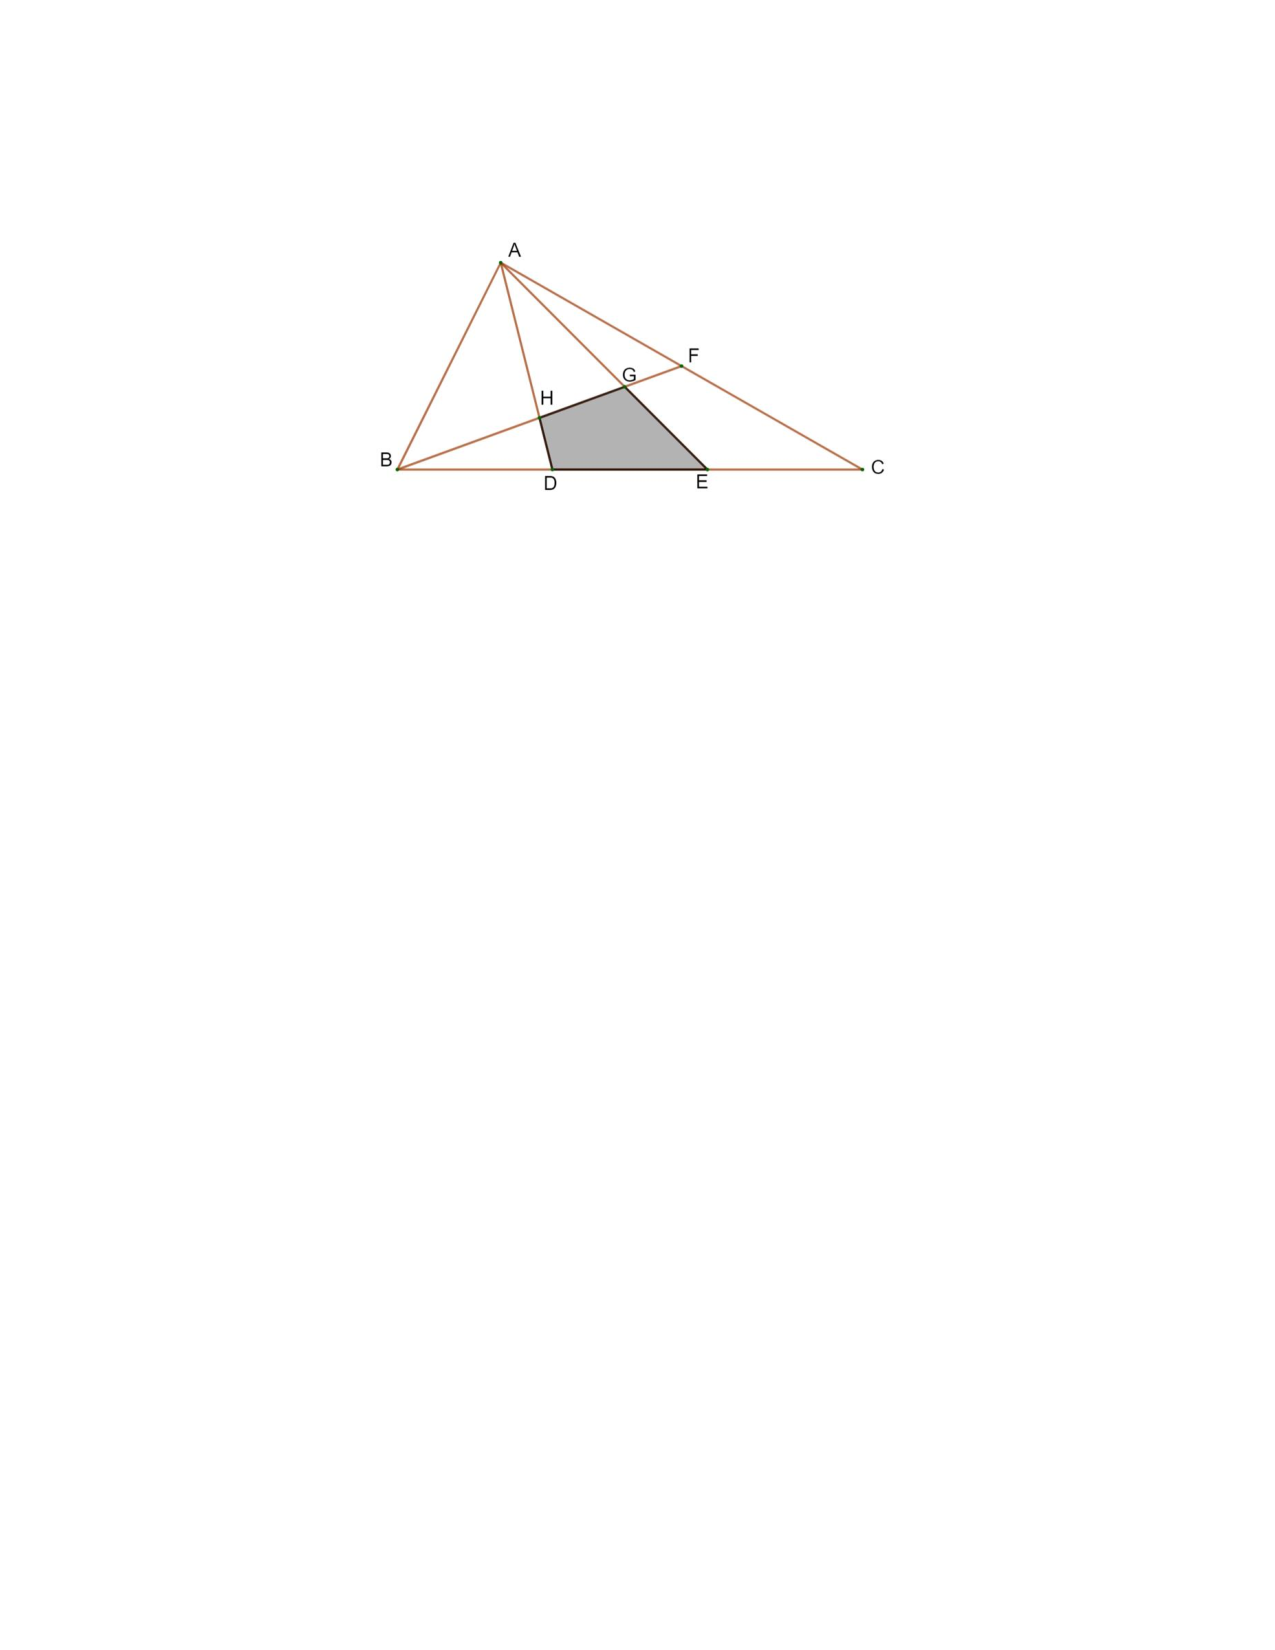
\includegraphics[width= 1\linewidth]{bai14k2}
%		\caption{\small\textit{\color{}}}
		\vspace*{-10pt}
	\end{figure}
	\textbf{\color{toancuabi}Bài} $\pmb{15.}$ Có bao nhiêu cách chọn ra $2$ số từ các số trong tập hợp $S=\{1,2,3,4,..,19,20\}$ sao cho tích của chúng là số chẵn?
	\vskip 0.1cm
	\textbf{\color{toancuabi}Bài} $\pmb{16.}$  Một số có ba chữ số được viết ngẫu nhiên. Xác suất để tổng các chữ số của số này bằng $5$ là bao nhiêu?
	\vskip 0.1cm
	\textbf{\color{toancuabi}Bài} $\pmb{17.}$ Có bao nhiêu số nguyên dương không lớn hơn $2024$ và nguyên tố cùng nhau với $2024$.
	\vskip 0.1cm
	\textit{(Hai số tự nhiên $(a,b)$ nguyên tố cùng nhau nếu $a$ và $b$ có ước chung duy nhất là $1$)}.
	\vskip 0.1cm
	\textbf{\color{toancuabi}Bài} $\pmb{18.}$ Cho hình vuông $ABCD$ và đường gấp khúc $CMNPQB$ như hình vẽ. Biết các độ dài $DM$, $MN$,
	$NP$, $PQ$ và $QB$ là $2$, $2$, $2$, $1$, $3$ đơn vị. Tính diện tích
	hình vuông $ABCD$.
	\begin{figure}[H]
		\vspace*{-5pt}
		\centering
		\captionsetup{labelformat= empty, justification=centering}
		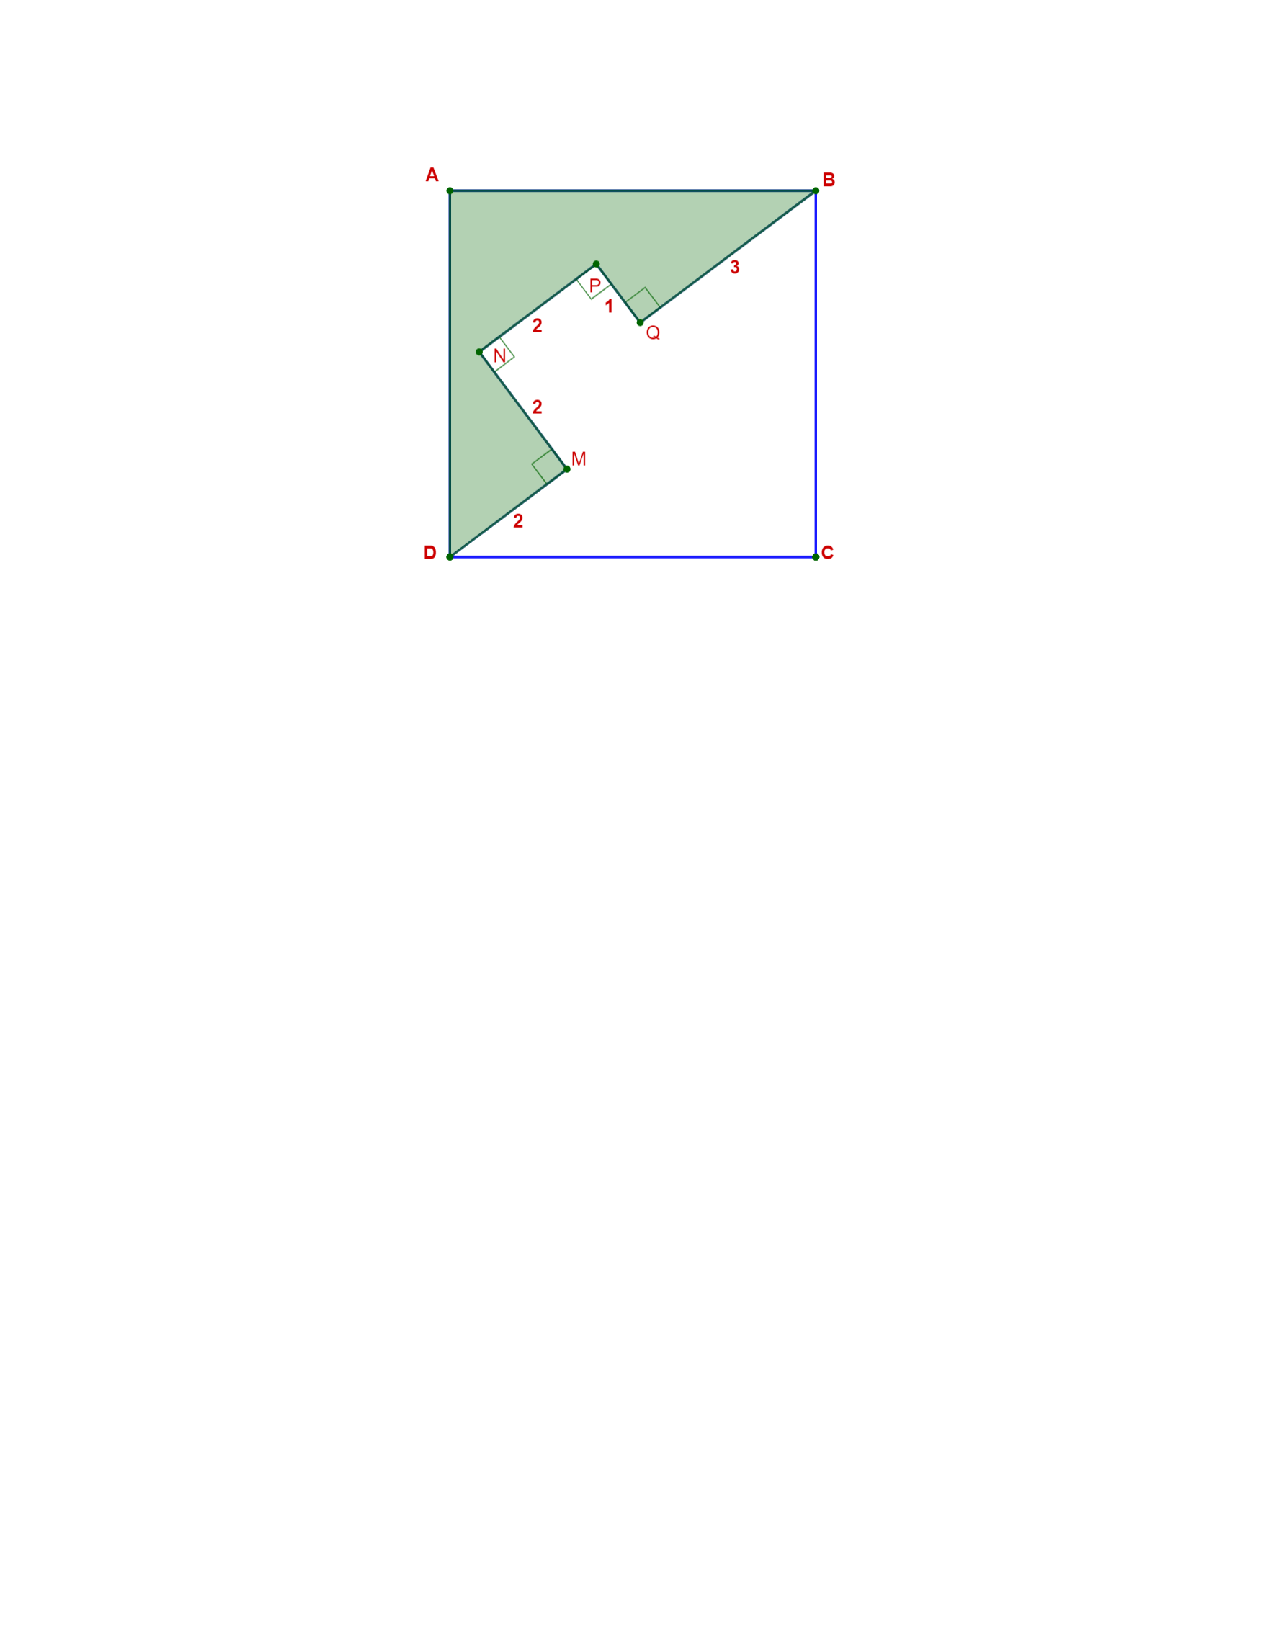
\includegraphics[width= 0.7\linewidth]{bai10}
		%		\caption{\small\textit{\color{}}}
		\vspace*{-10pt}
	\end{figure}
	\textbf{\color{toancuabi}Bài} $\pmb{19.}$ Ba số được chọn ngẫu nhiên từ $20$ số $\{1,2,3,..,20\}$. Xác suất để tổng ba số này chia hết cho $3$ là bao nhiêu?
	\vskip 0.1cm
	\textbf{\color{toancuabi}Bài} $\pmb{20.}$ Trong lễ bế giảng năm học mới, bạn Mạnh Quân được giao nhiệm vụ mua $20$ quả bóng bay về để trang trí lớp. Cửa hàng có $4$ loại bóng bay gồm các màu Xanh, Đỏ, Tím, Vàng. Có bao nhiêu cách mua $20$ quả bóng bay các màu nếu Mạnh Quân muốn mua mỗi màu số bóng bay ít nhất bằng $\frac{1}{5}$ số bóng bay cần mua?
\end{multicols}